\subsection{Generalizability of the Knowledge Graph}
A key question in building a knowledge graph is how useful it is in terms of generalizing to new programs.  To test the applicability of this knowledge graph to any sort of usage of it, we performed a ten fold cross validation study, where we split the test programs into 10 roughly equivalent sets, based on the total number of turtles we had found in our analysis of all programs.  Each set contained 51,371 turtles.  The actual number of program files included in each set ranged from 590-724 files.  We rotated each set as a `test set' of programs that we could generalize to, while building a `knowledge graph' from the remaining nine sets of program files.  Specifically, we examined whether each control flow and data flow edge in the `test set' of programs existed in the knowledge graph constructed from the other nine sets.  

Figure~\ref{hits_misses} shows the number of hits and misses for the test programs for control flow and data flow edges across the ten different splits, the X axis being the specific validation split.  Table~\ref{cross_validation_results} shows the results averaged across the same 10 `test' program sets.  The average number of control flow and data flow edges summed across test program files was 63,650.7 and 15,725.2 respectively, when the average was taken over 10 cross validation runs.  Across the ten sets of test programs, we found that the knowledge graph constructed from the remaining programs contained data flow edges from the `test' set 90.1\% of the time.  Similarly, 80.8\% of control flow edges in test programs were in the knowledge graph constructed from the remaining programs.  Overall, this means that the knowledge graph we constructed from GitHub programs generalize well to other unseen programs, in the sense that they contain most of the data flow and control flow edges we encountered in the test programs.

\begin{figure}
\centering
{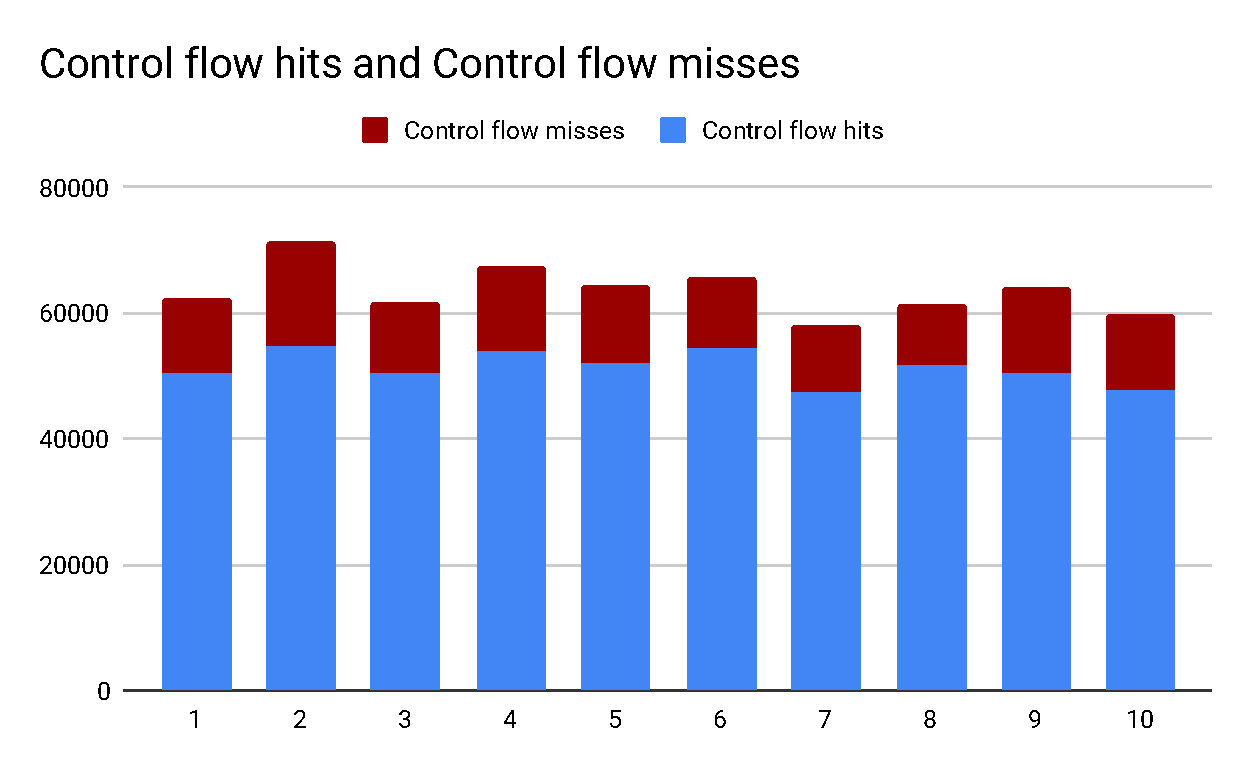
\includegraphics[width=0.48\textwidth]{control_flow_hits}}%
\hfill
{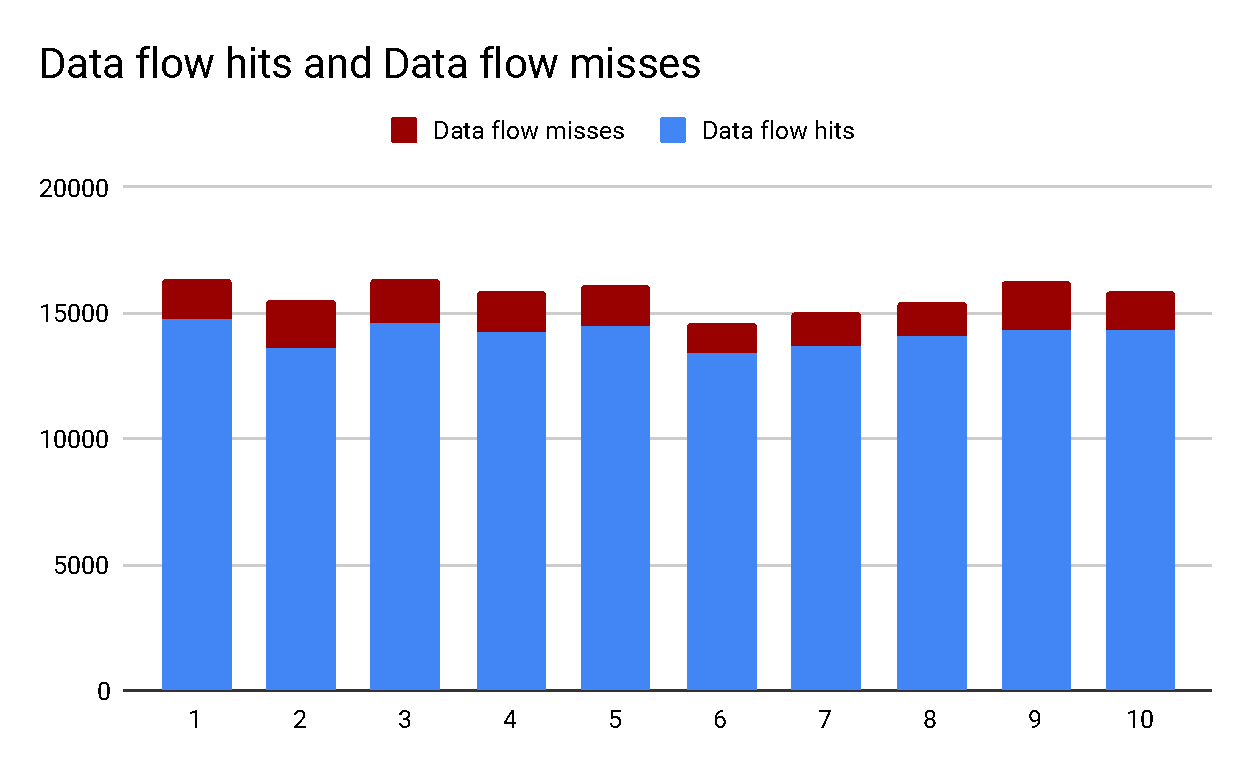
\includegraphics[width=0.48\textwidth]{data_flow_hits}}%
\caption{Hits versus misses for 10 splits}
\label{hits_misses}
\end{figure}


\begin{table}
\begin{center}
\begin{tabular}{ |l|l|} 
 \hline
Average number of control flow edges & 63650.7 \\
Average control flow percentage & 0.81 \\ \hline
Average number of data flow edges & 15725.2 \\
Average data flow percentage & 0.90 \\ \hline
\end{tabular}
\end{center}
\caption{Generalization of knowledge graph\\
to unseen test programs}
\label{cross_validation_results}
\end{table}

